To consider possibilities and limitations of the our approach we introduce an example machine learning streaming problem.

Let's suppose that we have an application that consists of the frontend and backend sides.
They both log user's queries and send logs to the log service.
For simplicity, let's assume that every user query produces one log entity from the frontend and one log entity from the backend, and they have equal and unique query id.

The log entities have the following structure (ts stands for the timestamp):

\begin{tabular}{|l|lllll|}
    \hline
    \textbf{frontend} & id & version & queryId & userId & ts \\
    \hline
\end{tabular}

\vspace{0.1em}

\begin{tabular}{|l|lllll|}
    \hline
    \textbf{backend} & id & queryId & userId & ts & payload \\
    \hline
\end{tabular}

We want to aggregate statistics about the time that authorized users from new frontend client versions wait for the application answer per user session.
To evaluate when the session ends we will use machine learning model that requires frontend features and user features.

One of the possible solutions is represented on the image TODO(image ref).
Obviously, this solution is not optimal.
Filters are applied to streams too late and number of partitions potentially can be reduced.
To be able to fix it safely we need to know about the requirements and impact of the each operation.

TODO what is triggers? \\
TODO stateful maps?

\begin{itemize}
    \item \textbf{joinByQueryId}: Requires queryId field in the elements of the both input streams.
    \item \textbf{addUsersFeatures}: Stateful map operation. Requires partition by userId. Users should not be filtered before to get valid statistics here. Adds userFeatures field to elements.
    \item \textbf{addFrontFeatures}: Stateful map operation. Requires only new front versions, adds frontFeatures field to elements in the stream.
    \item \textbf{filterNewFronts}: Filters elements with new front versions. Needs versionId in the input stream.
    \item \textbf{modelInference}: Stateful map operation. Requires front and users features. Sets trigger that signals when to emit data from aggregation. Users should not be filtered.
    \item \textbf{filterAuthorizedUsers}: Requires users features. Filters users that are authorized.
    \item \textbf{stats}: Requires authorized users from the new front versions. Also needs session trigger to be set. Sends accumulated statistics to the dashboard.
\end{itemize}

TODO SQL proof\\
We see here complex pipeline with stateful operations and triggers management.
So it is not possible to describe it in SQL.
Moreover, we see non-trivial operation requirements here, so concrete execution graph specification will not provide space for optimizations.

Let's consider another pipeline that satisfies requirements: TODO (image ref).
We can see that filters here are maximally close to data sources.
And after permutation of stateful operations we have one less data partition that is rather expensive operation.

In section \ref{sec:eval} we will specify this problem using contract-based approach and will see, how it helps in optimizations.

TODO insert image properly \\
TODO add to image ops naming \\
TODO split images \\
\begin{figure}
    \centering
    \label{fig:running-example-suboptimal}
    \label{fig:running-example-optimal}
    % Haskell 3 graph
    % Haskell 11 graph
    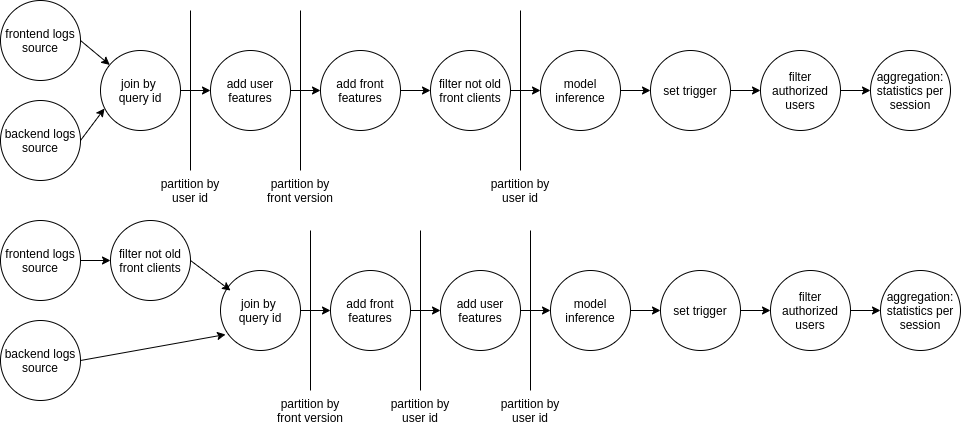
\includegraphics[width=\linewidth]{images/debs-calco-example}
\end{figure}
